\documentclass{article}
\usepackage{geometry}
\usepackage{fancyhdr}
\usepackage{amsmath, amsthm, amssymb}
\usepackage{graphicx}
\usepackage{hyperref}
\usepackage{color}
\usepackage{listings}
\lstset{ %
language=C++,                % choose the language of the code
basicstyle=\footnotesize,       % the size of the fonts that are used for the code
numbers=left,                   % where to put the line-numbers
numberstyle=\footnotesize,      % the size of the fonts that are used for the line-numbers
stepnumber=1,                   % the step between two line-numbers. If it is 1 each line will be numbered
numbersep=5pt,                  % how far the line-numbers are from the code
backgroundcolor=\color{white},  % choose the background color. You must add \usepackage{color}
showspaces=false,               % show spaces adding particular underscores
showstringspaces=false,         % underline spaces within strings
showtabs=false,                 % show tabs within strings adding particular underscores
frame=single,           % adds a frame around the code
tabsize=2,          % sets default tabsize to 2 spaces
captionpos=b,           % sets the caption-position to bottom
breaklines=true,        % sets automatic line breaking
breakatwhitespace=false,    % sets if automatic breaks should only happen at whitespace
escapeinside={\%*}{*)}          % if you want to add a comment within your code
}
\begin{document}

\title{Cryptographic Analysis}
\author{Colin Rice
    \and Samuel Milito
    \and Jacob Shedd}

\maketitle

\section{Flaws and Exploit Enablers}
There are a number of issues that, while not exploits in and of themselves, either allow exploits, or are issues within the system.

\subsection{Bank Deposit Limits}
Due to the incorrect way atm limits are implemented, completely on the server side and globally, the bank is limited to depositing 1000\$ into any account. It cannot make multiple 1000\$ deposits.

\subsection{Poor Scaling}
While not an issue with the current scale of the project, all account information is stored in a vector. With O(n) lookups, this will become incredibly slow with very large amounts of users.

\subsection{Overly Generous Timeouts}
The timeout checking on both sides is overly generous. The ATM has a 30 second window
\begin{lstlisting}
if(time(NULL) - messageTimeout < 30) // Bank Response needs to be in less that 30 seconds.
{
    // [...]
}
\end{lstlisting}
and the bank has no timeout handling at all. As such, packets can be held up to 30 seconds before being sent to the ATM, and indefinitely before being sent to the bank. This opens it up to much longer analysis than otherwise. While there is no specific exploit I have in mind, this is a much larger window than is needed for packets to be sent and received. In the proxy, a large amount of work can be done. Adding the following code in between receiving an ATM packet and forwarding the packet to the bank results in proper operation:
\begin{lstlisting}
printf( "Sleeping for 29 seconds.\n" );
sleep( 29 );
\end{lstlisting}
An example of adding the sleeps is below.
\\
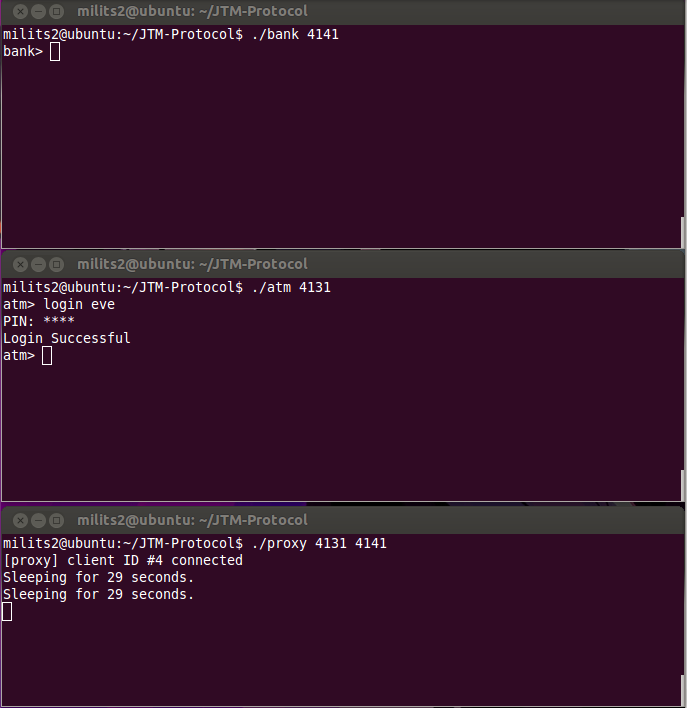
\includegraphics[scale=0.5]{slowLogin.png}
\\

\subsection{Lack of Server Side Verification}
On the server side, no verification is done that the received numbers are integers.
\begin{lstlisting}
    float b = (float)atof(info.at(4).c_str());
\end{lstlisting}
Bank balances should always be integers; there is no reason to accept floats.

\subsection{Bank Deposits Floats}
While the ATM only allows withdrawals of integer amounts, the bank allows for deposits of floats. There is no server side input verification other than making sure that it is a positive float. If there is a deposit at the bank with at least seven decimal places (e.g., 0.9999999), when the user checks their balance it will register as \$1 more than they previously had. They will then be able to withdraw the new amount, plus the dollar.

While this isn't very exploitable (the user would need to sit down at a bank's computer and deposit \$0.9999999 multiple times), it shows that the bank allows for malformed inputs.

In the following impage, repeated deposits of \$0.9999999 were followed by depositing a whole amount. This rolled it over, and allowed the user to withdraw the whole dollar amount.
\\
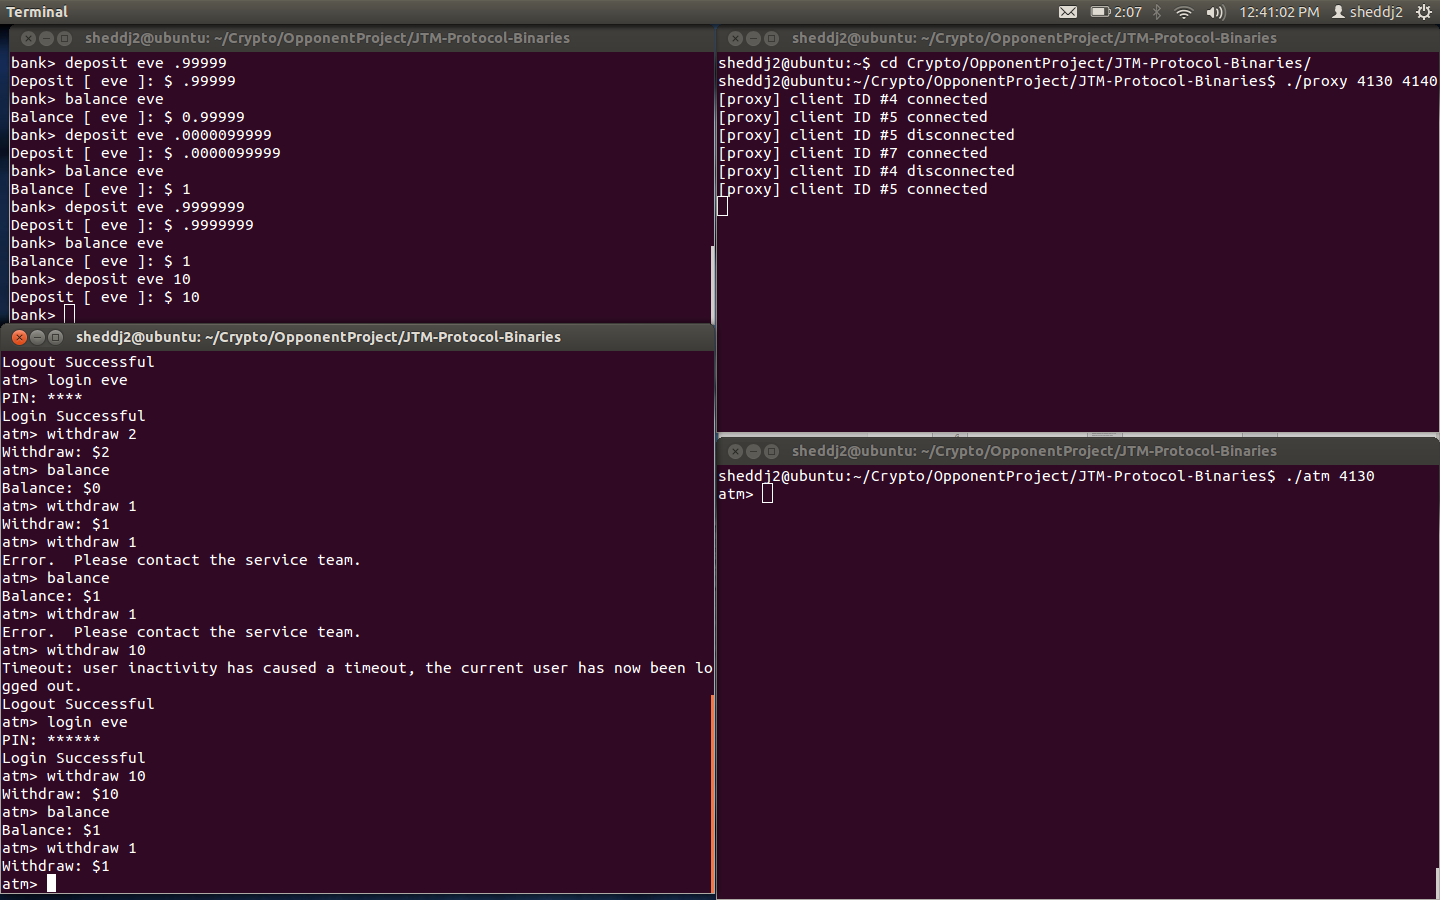
\includegraphics[scale=0.25]{StrangeFloatBehavior.png}
\\

\subsection{Single Line Login}
Example
\\
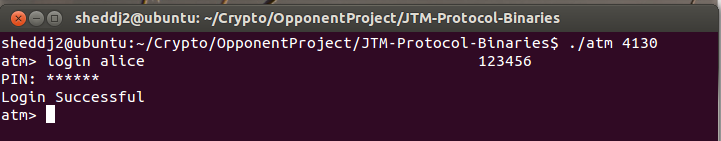
\includegraphics[scale=0.5]{OneLineLogin.png}
\\
Because of the way the atm parses user input it is possible to have the user login and pin on the same line. This still allows the user to login but for anyone looking over their shoulder they would see the pin in cleartext.

\subsection{Poor PIN Verification}
PINs are supposed to be 6 characters, but any amount of zeros at the end are ignored. If a PIN is entered with less than the required characters, it pads it out with zeros:
\begin{lstlisting}
pin = getPin("PIN: ");
pin = pin.substr(0,6);
while(pin.length() < 6)
{
    pin = pin + "0";
}
pin = toNumbers(pin);
\end{lstlisting}
For example, a PIN of 678900 will accept 6789, 67890, or 678900.

\subsection{Key Management}
The binaries do not have hardcoded keys. Instead of being cooked into the binaries, they read the keys from a special folder. This has two consequences. First, it makes it far easier to get copies of the keys. Second, it allows for on-the-fly key manipulation--if an attacker has access to the directory controlling the keys, they can be changed at runtime.

\subsection{No HMAC}
There is no HMAC being used. Messages are hashed, but it is simple SHA512, which is not passworded. If the encryption is broken, modifying a message is trivial, as the attacker can just recompute the hash.

\subsection{Unhashed Card Contents}
The card contents are never hashed. There is a getCardHash function that does no hashing:
\begin{lstlisting}
std::string getCardHash(std::string cardFile) 
{
    std::ifstream card(cardFile.c_str());
    std::string tempHash((std::istreambuf_iterator<char>(card)),std::istreambuf_iterator<char>());
    
    std::string cardHash = tempHash;
    cardHash = cardHash.substr(0,128);
    std::transform(cardHash.begin(), cardHash.end(), cardHash.begin(), ::toupper);
    cardHash = toHex(cardHash);
    
    return cardHash;
}
\end{lstlisting}
It just reads the first 128 characters from the file (or attempts to, there is no assurance that it has 128 characters) then converts it to uppercase, then lastly to hex. Note that the toHex function does no verification on the string; if it's fed invalid hex it just replaces all characters not 0-9, A-F with 0.
\begin{lstlisting}
std::string toHex(std::string inputStr)
{
    std::string retStr = "";
    for(int i = 0; i < inputStr.length(); i++)
    {
        if(('0' <= inputStr[i] && inputStr[i] <= '9') || ('A' <= inputStr[i] && inputStr[i] <= 'F'))
        {
            retStr += inputStr[i];
        }
        else
        {
            retStr += "0";
        }
    }

    return retStr;
}
\end{lstlisting}

\subsection{RNG Flaws}

Their random number generator when asked for 32 bytes of data outputs 32
random hex bytes. This means that each byte only has 16 ($2^{4}$) possibilities instead
of 256 ($2^{8}$).

The end result is that everything generated using these functions (AES keys, nonces, etc.) only
have 128 bits of randomness instead of the expected 256 bits of randomness.
\begin{lstlisting}
std::string getRandom(int length)
{
     std::string retStr = "";
     CryptoPP::AutoSeededRandomPool rng;
     int random;
     int num = 0;
     bool hex = true;

     for(unsigned int i = 0; i < length; ++i)
     {
         random = (int) rng.GenerateByte();
         if(hex)
         {
             // Generate Random Hex String
             num = (int) (random % 16);
             if(num < 10)
             {
                 retStr += (num + '0');
             }
             else
             {
                 retStr += ((num - 10) + 'A');
             }
         }
         else
         {
             // Generate Random String With ASCII Range (48, 126)
             num = (int) (random % (126 - 48));
             retStr += (num + '0');
         }
     }

     return retStr;
}
\end{lstlisting}

\section{Exploits}

\subsection{Invalid Transfers}
A transfer to an invalid user succeeds initially, as the checks are done out of order, namely the highlighted lines:
\begin{lstlisting}
bool processTransfer (std::vector<std::string> info)
{
	float b = (float)atof(info.at(4).c_str());
	if(b > 1000.00) {
		return false;
	}

	std::vector<Account>::iterator it;
	for (it = Database.begin(); it != Database.end(); it++) {
		if(it->get_un() == info.at(1) && it->get_logged_in() && b <= it->get_balance() && it->get_transfer() + b <= 1000.00) {
===>		it->reduce_balance(b);
===>		it->increase_transfer (b);
			std::vector<Account>::iterator foo;
			for (foo = Database.begin(); foo != Database.end(); foo++) {
				if(foo->get_un() == info.at(5) && foo->get_balance() + b <= MAX_BAL) {
					foo->increase_balance (b);
					return true;
				}
			}
		}
	}
	return false;
}
\end{lstlisting}
The active user has their account debited before the targetted user has their account credited. The result is that issuing a transfer to an invalid user will result in the active ATM user losing money, which then vanishes entirely from the system. In the image, Bob has \$40 vanish when he attempts to transfer it to Vriska, a nonexistant user.
\\
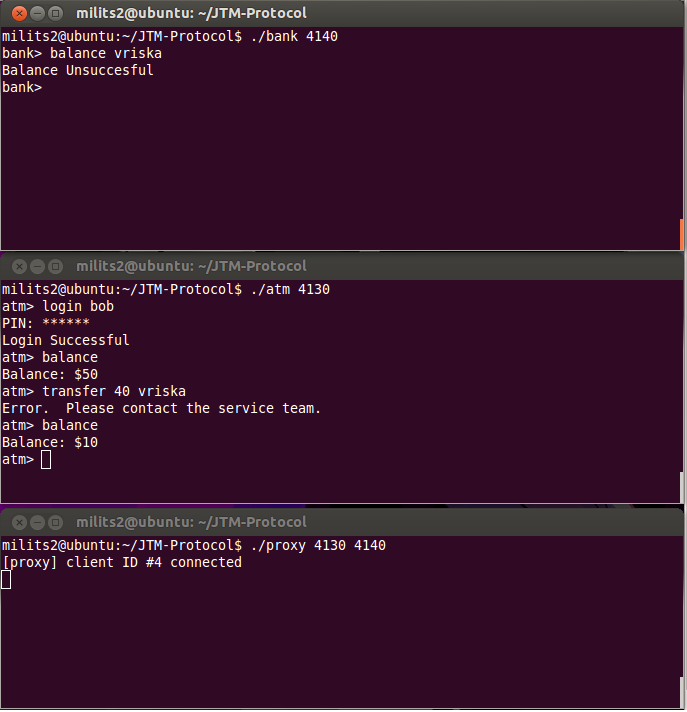
\includegraphics[scale=0.5]{transferLoss.png}
\\

\subsection{Account Enumeration Via Transfer}
\$0 transfers can be used to verify whether or not a given user has an account at the bank. For example, Alice tries to send \$0 to Eve (which succeeds) and Vriska (which fails), showing that Eve has an account, but Vriska does not. In the image, Alice verifies that Bob is a valid user (as the transfer succeeds) and that Vriska is not a valid user, as the transfer fails.
\\
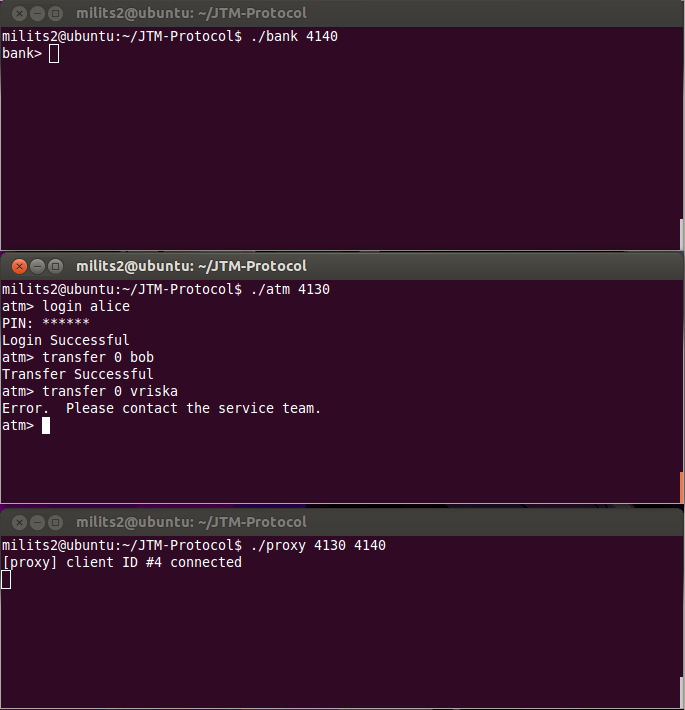
\includegraphics[scale=0.5]{transferUser.png}
\\

\subsection{Dysfunctional Card Verification}
The actual contents of a card file are ignored. The only verification done on the card is if it has anything in it. That is, any card put into the machine will satisfy it, as long as it doesn't have a blank "magnetic strip" (i.e., contents). This is a massive security flaw, as it is a failure of two-factor security. 128 characters are read from the card file, and summarily ignored (after being sent as encrypted plaintext). The login code is as follows:
\begin{lstlisting}
bool login (std::vector<std::string> info) 
{
	std::vector<Account>::iterator it;
	int pin = atoi(info.at(3).c_str());

	for (it = Database.begin(); it != Database.end(); it++) {
		if(it->get_un() == info.at(1) && it->get_pin() == pin && !it->get_logged_in() && !it->get_locked()) {
			it->set_logged_in_true ();
			return true;
		} 
		else if(it->get_un() == info.at(1) && it->get_pin() != pin && !it->get_logged_in()) {
			it->increase_login_attempts();
			if(it->get_login_attempts() >= 3) {
				it->lock();
			}
			return false;
		}
	}
	return false;
}
\end{lstlisting}
It verifies that the PIN matches, but never checks if the card actually matches with anything. In fact, the card is never used anywhere. The only verification on the card is that the file exists and isn't empty:
\begin{lstlisting}
if(cardFile)
{
    sendPacket = true; 

    username = temp;

    cardHash = getCardHash(cardFilename);

    pin = getPin("PIN: ");
    pin = pin.substr(0,6);
    while(pin.length() < 6)
    {
        pin = pin + "0";
    }
    pin = toNumbers(pin);
}
else
{
    temp = "";
    cout << "ATM card not found.\n";
}
\end{lstlisting}
This verifies that the card exists, and that is all. The card is eventually rolled into a packet (see below) then never used.

\subsection{Permanent Lockout}
If a user fails their login three times, they are permanently locked out at all ATMs forever. If a login fails due to incorrect PIN, it progresses towards a lockout:
\begin{lstlisting}
it->increase_login_attempts();
if(it->get_login_attempts() >= 3) {
	it->lock();
}
\end{lstlisting}
Once an account gets locked, it's locked for all ATMs on a permanent basis. In the below picture, the lower ATM failed a login three times, and the one above it was unable to log in, even though it used the correct PIN.

\subsection{Login Info}
All login info is sent in cleartext inside the encrypted packet. The most 
significant issue is that the PIN is sent unencrypted. The first 128 characters 
in the card file are sent, regardless of if the card file contains 128 characters 
or not. Note that the card contents are ignored. 

None of the login information is hashed, so being able to decrypt messages reveals 
the full amount of information needed to compromise somebody's account. As it also 
sends account name, an attacker has account name, PIN, and the (unused) card number.
\begin{lstlisting}
void* formATMPacket(char packet[], std::string command, std::string username, std::string cardHash, std::string pin, std::string item1, std::string item2, std::string atmNonce, std::string bankNonce)
{
    std::vector<std::string> tempVector;
    tempVector.push_back(command);
    tempVector.push_back(username);
    tempVector.push_back(cardHash);
    tempVector.push_back(pin);
    tempVector.push_back(item1);
    tempVector.push_back(item2);
    tempVector.push_back(atmNonce);
    tempVector.push_back(bankNonce);
    formPacket(packet, 1023, tempVector);
}
\end{lstlisting}
The packet sent on login and all other requests contains the unhashed username, card/account number, and PIN.

\subsection{Crashing the Bank}
Adding a single line of code to the proxy will crash the bank. The bank cannot handle a malformed handshake message. The follow section of code in the proxy:
\begin{lstlisting}
while(1)
{
	//read the packet from the ATM
    // [...]
	
	// Crashes bank
    strcpy( packet, "" );
    
	//forward packet to bank
    // [...]
	
	//get response packet from bank
    // [...]
	
	// Crashes ATM
	strcpy( packet, "" );
	
	//forward packet to ATM
    // [...]
}
\end{lstlisting}
can be easily manipulated to crash the bank (or, similarly, the ATMs, as detailed slightly later). Adding the line of code before forwarding the packet to the bank crashes the bank as soon as an ATM user attempts to log in. 
\\
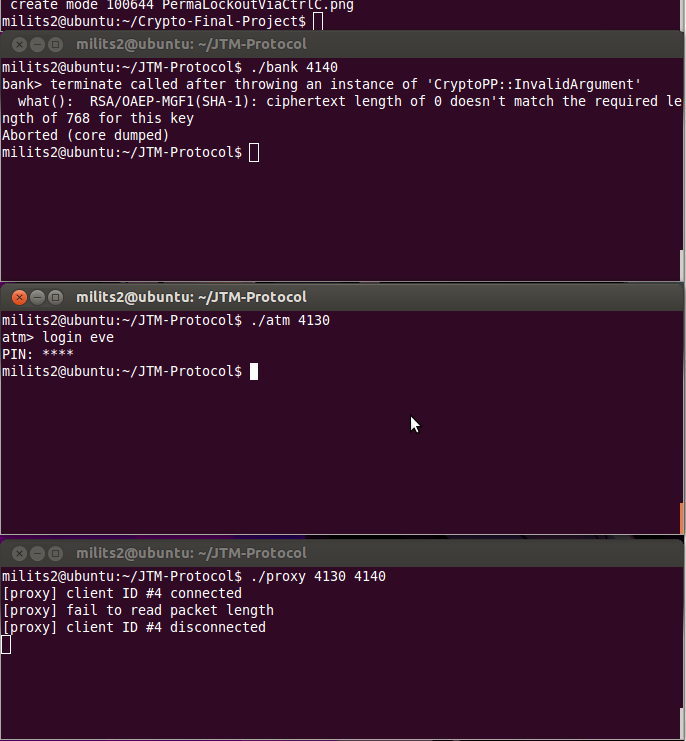
\includegraphics[scale=0.5]{crashBank.png}
\\
Similarly, ATMs can be crashed by adding the line of code before forwarding the packet to the ATM.
\\
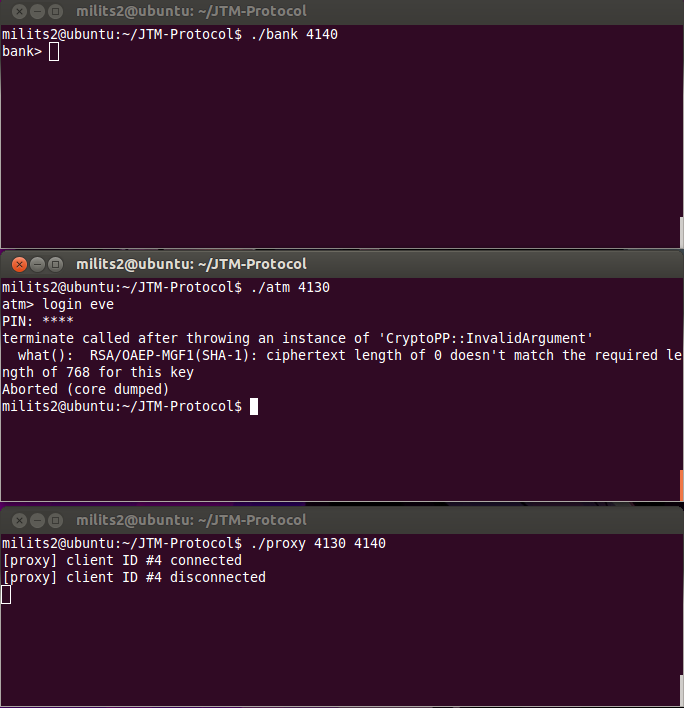
\includegraphics[scale=0.5]{crashATM.png}
\\
If both lines are left in, the bank crashes with a core dump, and the ATM crashes with no error message. This issue is due to not checking the validity of initial handshake messages. When it receives a blank message, it still tries to proceed with setting up a secure connection. The cryptographic functions crash, and the ATM and/or bank crash with them.

\subsection{Race Conditions}

The code as-is provides no protections on money, i.e., there are no mutex locks. For example, the withdrawl function:
\begin{lstlisting}
bool processWithdraw (std::vector<std::string> info)
{
	float b = (float)atof(info.at(4).c_str());
	if(b > 1000.00) {
		return false;
	}

	std::vector<Account>::iterator it;
	for (it = Database.begin(); it != Database.end(); it++) {
====>	if(it->get_un() == info.at(1) && it->get_logged_in() && b <= it->get_balance() && it->get_withdraw() + b <= 1000.00) {
			it->reduce_balance(b);
			it->increase_withdraw (b);
			return true;
		}
	}
	return false;
}
\end{lstlisting}
That is, a user logged on multiple times could theoretically withdraw double the amount in their account, assuming that the timing went through correctly. They would need to pass the marked line at the same time on two consoles, and it will authorize withdrawal on two ATMs, regardless if it would go over the account balance or the daily \$1000 limit. The only protection against this is not allowing users to log in on multiple machines at a time. However, the login function is also succeptible to a race condition:
\begin{lstlisting}
bool login (std::vector<std::string> info) 
{
	std::vector<Account>::iterator it;
	int pin = atoi(info.at(3).c_str());

	for (it = Database.begin(); it != Database.end(); it++) {
===>	if(it->get_un() == info.at(1) && it->get_pin() == pin && !it->get_logged_in() && !it->get_locked()) {
			it->set_logged_in_true ();
			return true;
		} 
		else if(it->get_un() == info.at(1) && it->get_pin() != pin && !it->get_logged_in()) {
			it->increase_login_attempts();
			if(it->get_login_attempts() >= 3) {
				it->lock();
			}
			return false;
		}
	}
	return false;
}
\end{lstlisting}
If the timing works out correctly, a user will pass all required checks (the highlighted line), and then set\_logged\_in\_true will be called. During this time, any other ATMs can then theoretically pass the same checks. The end result is that a single user would be logged on at multiple ATMs. Due to how fast all of the operations are (the data sets are miniscule), a demonstration was not feasible. This issue is exacerbated by the thirty second timeout window for packets (i.e., the bank accepts a packet if it's no more than 30 seconds old), as the proxy could hold packets, making sure that they are sent to the bank at identical times.

With a user logged on to multiple ATMs, they can abuse the race conditions to withdraw or transfer double their account balance.

\subsection{Handshake Hijacking}
When the bank and ATM establish a handshake, the ATM sends the bank a nonce encrypted with the bank's RSA key. The bank then sends back an encryption key and the nonce, as well as its own generated nonce. There is no explicit authentication.

Assuming an attacker has the ATM's public key, it is possible to masquerade as the bank. The attacker can simply send back a key encrypted with the ATM's public key and the nonce.

As there is no RSA (or other) authentication, if an attacker can guess the nonce, they can masquerade as the bank. Normally this would take $2^{256}$ attempts, but due to the aforementioned RNG flaw, it only takes $2^{128}$ attempts. Even worse, if the ATM is being run on an embedded system, entropy will be low upon startup, making it possible to guess the output of the system's random number generator.

If a successful masquerade is established, there are two crippling exploits, with some less important ones. The first is full account information obtained, as the proxy can then decrypt the message, which contains full cleartext login information for the user (see Login Info). The second is verifying all requests, including withdrawals for any amount. That is, masquerading as the bank compromises login information for all users who connect and also allows attackers to drain all of the money from any ATM.

\end{document}
